The given system of equations can be written the matrix equation form as
\begin{align}
    \vec{A}\vec{x}=\vec{b}\\
    \label{:solutions/det/52/A}
    \implies \myvec{1&2\\2&3}\myvec{x\\y}=\myvec{2\\3}
\end{align}
The augmented matrix for \eqref{A} is row reduced as follows
\begin{align}
    \myvec{1&2&2\\2&3&3}
    \xleftrightarrow[]{R_2\leftarrow R_2-2R_1}
    \myvec{1&2&2\\0&-1&-1}\\
   \xleftrightarrow[]{R_1\leftarrow R_1+2R_2}
    \myvec{1&0&0\\0&-1&-1}
    \xleftrightarrow[]{R_2\leftarrow (-1)R_2}
    \myvec{1&0&0\\0&1&1}\\
    \implies Rank\myvec{1&2\\2&3}=Rank\myvec{1&0&0\\0&1&1} =2
\end{align}
Hence, system of equations is consistent and has unique solution \myvec{0\\1}. See Fig. \ref{fig1:solutions/det/52/}

\begin{figure}[!ht]
\centering
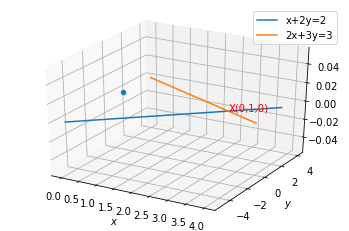
\includegraphics[width=\columnwidth]{./solutions/det/52/A2.png}
\caption{Intersection of lines x+2y=2 and 2x+3y=3}
\label{fig1:solutions/det/52/}
\end{figure}
